18. $y=\cfrac{|x+2|}{2+x}(x^2+4x+3)=\begin{cases}x^2+4x+3,\ x>-2,\\ -x^2-4x-3,\ x<-2.\end{cases}$
$$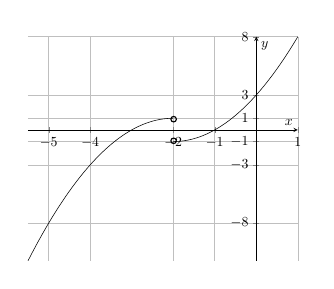
\begin{tikzpicture}[scale=0.5]
\begin{axis}[
    axis lines = middle,
    grid=major,
    legend pos={south west},
    xlabel = {$x$},
    %xlabel style={below right},
    ylabel = {$y$},
    xtick={-5,-4,-2, -1,1},
    ytick={-8, -3, 1, -1,8,3},
                  ]
	\addplot[domain=-5.5:-2, samples=100, color=black] {-x*x-4*x-3};
    \addplot[domain=-2:1, samples=100, color=black] {x*x+4*x+3};
	%\addlegendentry{$\text{Рис. 1}$};
\end{axis}
\draw (3.7,3.6) circle (2pt);
\draw (3.7,3.05) circle (2pt);
\end{tikzpicture}$$
